%!TEX root = ../main.tex
\section{Background}

\subsection{KBE-systems} % (fold)
\label{sub:kbe_systems}
Knowledge Based Engineering (KBE) is the art of using computerized knowledge to automate engineering design. KBE systems make the engineers able to write dedicated programs that preform complex and specific engineering task efficiently. It can, for example, take engineers weeks to iterate to a final design including geometry, simulations and documentation. With a KBE application the same work could be archived within days due to reuse of knowledge and design.

A clear and strict definition of KBE has proven almost impossible to define. The term is so broad that it is difficult to embrace all aspects. One good and suitable definition is written by Chapman, see Definition~\ref{def:kbe}.

\begin{mydef}
\label{def:kbe}
  KBE represents an evolutionary step in Computer-Aided Engineering (CAE) and is an engineering method that represents a merging of Object-Oriented Programming (OOP), artificial intelligence (AI) and Computer-Aided Design (CAD) technologies, giving benefit to customized or variant design automation solutions \citep{chapman}.
\end{mydef}


KBE is a combination of object-oriented programming and artificial
intelligence with computer aided design. It is designed to allow complex rules, heuristics, artificial intelligence and integration of other suitable systems. KBE is therefore more powerful and flexible then standard CDE/CAD systems.

KBE systems is often build on an open architecture \citep{chapman}. This enables the system to incorporate different software, like geometric kernels, CAD systems, FEA systems, databases, and graphical components. This makes the KBE system more suitable to be integrated in a product lifecycle process. Figure~\ref{fig:aml} show one possible architecture of the AML system.

\begin{figure}[ht!]
\centering
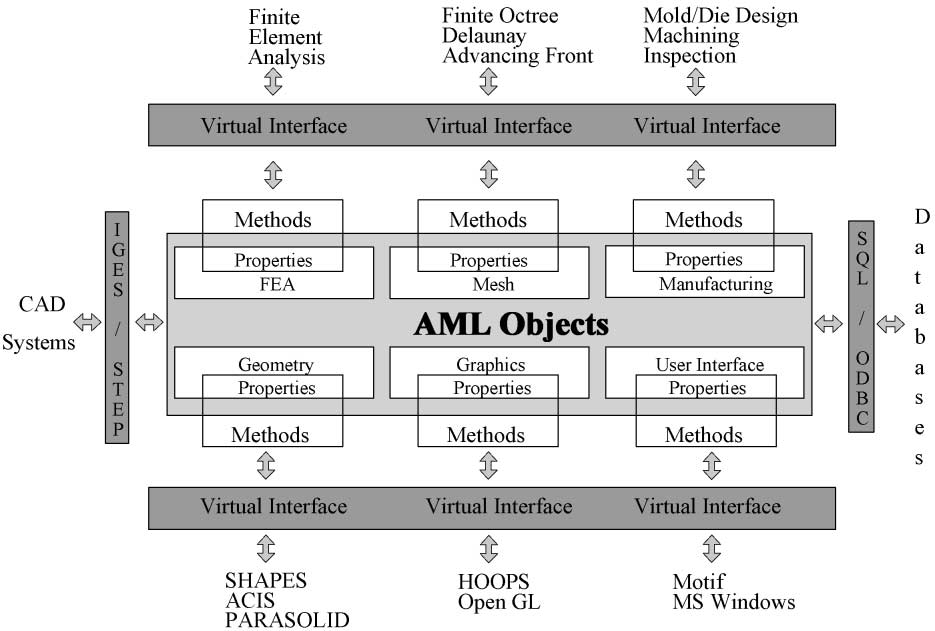
\includegraphics[width=110mm]{gfx/aml_program_structure.png}

\caption{AML virtual layer architecture \citep{AML}}
\label{fig:aml}
\end{figure}

% subsection kbe_systems (end)

\subsection{Modern general software development tools} % (fold)
\label{sub:modern_general_software_development}


General Software Development (GSD) is a synthesis of many disciplines. From modeling, design, code generation, project management to testing, debugging and deployment. The variety makes software development a complex and often a difficult task. Through the last decade software development has come a long way in trying to minimize this complexity. General software development tools form an important component of this evolution. These tools have particularly made an impact in the robustness, portability, re-usability and effectiveness in the software development.

%The GSD tools is related to the term Computer-aided software engineering (CASE) tools, but embraces not as much.
GST tools is designed to help a developer with repetitive and time consuming tasks. Debugging, testing, creating and maintaining code are some of these tasks. The term is usually used about relatively simple programs that can be used in many different software development environments.

 \begin{mydef}
  \label{def:GST}
  General software development tool is a program that software developers use to create, debug, maintain, or otherwise support other programs and applications.
\end{mydef}


These tools are used in modern software development environments. They are often general, which means they can be used om many different development environments. Some examples are testing frameworks, debuggers, and IDE's. .

 \subsubsection{Test Framework} % (fold)
 \label{ssub:test_framework}

 % subsubsection test_framework (end)
Testing frameworks makes the developer able to test, maintain and control the quality of his code. Is is an execution environment for automated tests and is the overall system in which the tests will be automated.

\begin{mydef}
  \label{def:testing_framework}
  Testing Framework is the set of assumptions, concepts, and practices that constitute a work platform or support for automated testing.
\end{mydef}

From definition~\ref{def:testing_framework} we can conclude that the testing framework is responsible for:

\begin{itemize}
  \item Defining how the express expectation should be formated.
  \item Executing the tests.
  \item Reporting results.
  \item Creating a mechanism to drive the application under test.
\end{itemize}

In short Test frameworks helps teams organize their test suits in turn to help improve the efficiency of testing.

\subsubsection{Debugger} % (fold)
\label{ssub:debugger}
 Typically a debugger offers a lot of different features. Some of these features are step-by-step execution, symbol resolver, breakpoints, GUI interface and so on. It is used to examine a program for errors and it is a exceptionally practical software tool.

\begin{mydef}
\label{def:debugger}
A debugger is special program used to find errors in other programs. A debugger allows a programmer to stop a program at any point, examine the code and variables and change the values of variables.
\end{mydef}

Debuggers are normally used to find error and bugs in the code base, but can also be used to get a better understanding of the code base. One can for example follow a variable or object through different transformations throughout the program execution.
% subsubsection debugger (end)

\subsubsection{Integrated Development Environment} % (fold)
\label{ssub:ide_support}
An Integrated Development Environment (IDE) is a software application that provides comprehensive facilities to a software developer. It combine many features of different tools into one package. An IDE can for example provide a text editor, a compiler and/or interpreter, text and file search, a debugger, test runner, and other efficiency enhancing features.

% Some words about general software engineering practices.
% subsection modern_general_software_development (end)

\subsection{Combining KBE and general software development} % (fold)
\label{sub:combinding_kbe_and_general_software_development}
%Motivation for doing this work.

Todays KBE tools have proven itself to be able to produce solutions of great value. The demand for new solution and further development is increasing. This increase in demand has reviled some challenges in terms of code maintenance, code quality and make the application not only accessible for ‘‘natural born hackers’’ \citep{rocca}. The solution can be based on a more advanced developer environment with more support tools and better methodologies.

GSD has today come a long way in terms of environment, support tools and work methodologies. Developers and project planers can pick and choose from a range of different utilities. The tools are portable and can be used by all kinds of development. This evolution started in the 80's by the academic community. When the software industry, in the 90's, started to acknowledge the need the evolution flourished. Through the 1990's and 2010's the software industry saw a boost in productivity, efficient, code quality, project control, coordination within the programming groups and speed to delivery \citep{case_tools}.


KBE development, on the other hand, is today based around special-purpose modeling frameworks and programming languages. This makes the portable GSD tools not as easily integrable. While the KBE development has been very successful, there is steel room for improvement. There is today a lot of tools that is not implemented in the KBE environment, that in the software industry has made a deep impact.

%[TODO Skal vi si noen om at Likheten er stor...]

This gap between KBE development and GSD is recognized by many KBE industries today. KBeDesign at Aker Solution has one of these companies. They have investigates many possibilities and tools, like contionous integration and control version systems. They are also trying to implement a testing framework for the AML environment. This framework is AUnit and started as a master thesis at the Norwegian University of Science and Technology (NTNU) \citep{aunit}.





%Since the KBE environment has a proprietary environment that don't have a wide community, it cannot as easily follow the evolution as the rest of GSD. Every tool has to be made and tested, which makes integrating GSD tools a time consuming project.



% We see that programming environments that have a great community get benefits from each other. One of this communities is the python programming language, which have a lot of GSD tools in its environment.


% This Id the gap we vil try to investegate. is it so hard and time consuming to integrate GST in the KBE envoronment.

%from \citep{case_tools}
%Their research also shows clearly that the above abilities of CASE tools can certainly simplify the maintenance of such projects by enforcing a software engineering standard and while at the same time enabling a general uniformity in the design and development phases.


% subsection combinding_kbe_and_general_software_development (end)
